\documentclass[10pt,conference]{IEEEtran}
\usepackage{cite}
\usepackage{graphicx}
\usepackage{booktabs}
\usepackage{url}
\usepackage{array}
\usepackage{amsmath}
\usepackage{placeins}
\usepackage{hyperref}

\graphicspath{{../figures/}}
\setlength{\textfloatsep}{8pt plus 1pt minus 2pt}
\setlength{\floatsep}{8pt plus 1pt minus 2pt}
\setlength{\intextsep}{8pt plus 1pt minus 2pt}
\renewcommand{\topfraction}{0.95}
\renewcommand{\dbltopfraction}{0.95}
\renewcommand{\textfraction}{0.05}
\renewcommand{\floatpagefraction}{0.85}
\renewcommand{\dblfloatpagefraction}{0.85}

\title{A Patient-Wise CHB-MIT Seizure Prediction Study with Leakage, Label, and Horizon Audits}
\author{\IEEEauthorblockN{Boppidi Anish Reddy, Avanika Kademgari, and Trupti Kudale}}

\begin{document}
\maketitle

\begin{abstract}
Seizure prediction from scalp EEG is difficult to evaluate because patient leakage, class imbalance, overlapping windows, and broad preictal label definitions can produce misleading estimates of performance. This study reports a repository-backed, patient-wise CHB-MIT seizure prediction pipeline and uses completed experiments to examine whether model choice, imbalance handling, or preictal horizon length explains poor discrimination. The frozen dataset contains 10 CHB-MIT patients, 273 EDF recordings, 50 annotated seizures, and 734,796 four-second windows. Each EDF was processed with 18 common EEG channels, 0.5--40 Hz bandpass filtering, 50 Hz notch filtering, 4 s windows with 2 s stride, per-window z-score normalization, a 10 min preictal definition, and a 60 s postictal exclusion interval. EEGNet achieved validation PR-AUC 0.0239 and F1 0.0366; Attention achieved validation PR-AUC 0.0258 and F1 0.0000; and the time-limited Hybrid run achieved validation PR-AUC 0.0238 and F1 0.0461. The label audit found no evidence of mechanical label contamination under the implemented checks, but 47.26\% of positive windows occurred more than five minutes before seizure onset. A controlled preictal horizon ablation over 10, 7.5, 5, and 3 min did not produce a shorter horizon that improved both validation PR-AUC and validation F1 over the 10 min baseline. These results do not support claims of clinical readiness or state-of-the-art performance; instead, they provide an audited negative result showing that simple imbalance handling and global horizon shortening were insufficient under this patient-wise protocol.

\end{abstract}

\section{Introduction}
Epileptic seizure prediction seeks to identify a preictal state before clinical seizure onset. Public electroencephalography (EEG) datasets such as the Children's Hospital Boston--Massachusetts Institute of Technology (CHB-MIT) Scalp EEG Database enable reproducible benchmarking \cite{physionet_chbmit,goldberger2000physiobank}, but the task is unusually sensitive to experimental design. Patient leakage can inflate performance, overlapping windows can reduce the effective number of independent samples, and the definition of ``preictal'' can convert a physiologically uncertain interval into a hard binary label \cite{mormann2007seizure,kuhlmann2018seizure}.

This paper reports a completed and frozen CHB-MIT study whose main contribution is not a high-performing model, but an audited experimental account of what did and did not work under a patient-wise protocol. We ask whether standard imbalance strategies, attention or hybrid architectures, or shorter global preictal horizons improve patient-wise window-level discrimination. Under the completed protocol, none of these changes produced strong validation area under the precision-recall curve (PR-AUC) or F1. We therefore frame the study as a reproducibility and problem-formulation contribution rather than a performance benchmark.

Figure~\ref{fig:pipeline} summarizes the complete repository-backed workflow. Later figures show the data flow, preprocessing, and training components used to organize the completed experiments.

\begin{figure}[!t]
\centering
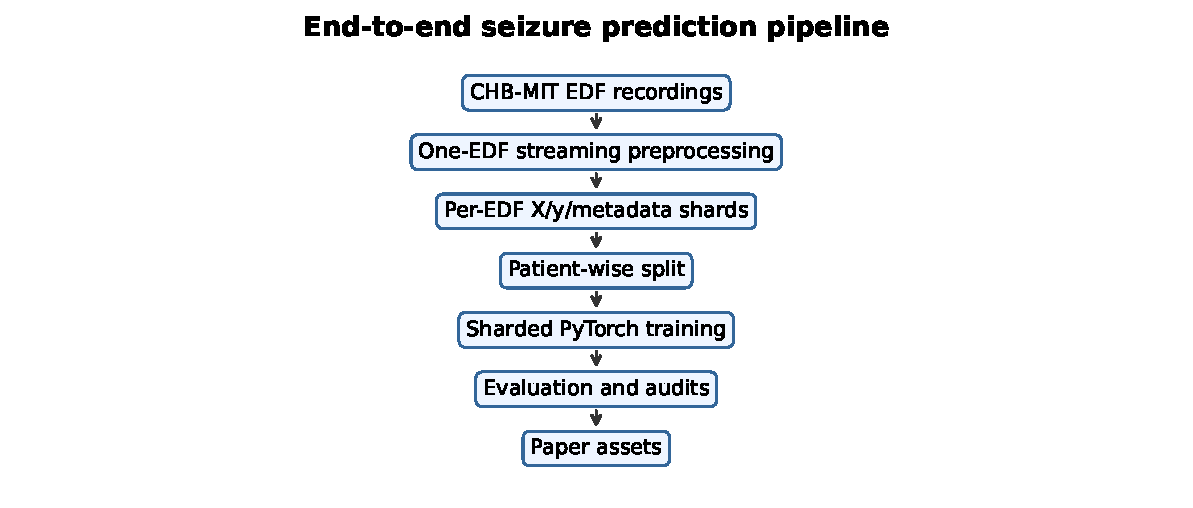
\includegraphics[width=\columnwidth]{pipeline_diagram.pdf}
\caption{End-to-end pipeline from CHB-MIT EDF recordings to paper artifacts. The workflow documents the audited processing, training, evaluation, and reporting path and does not imply clinical deployment.}
\label{fig:pipeline}
\end{figure}

\section{Related Work}
CHB-MIT seizure-prediction studies differ in window length, feature representation, preictal horizon, seizure prediction horizon, seizure occurrence period, and patient-specific versus patient-independent evaluation \cite{truong2018cnn,dissanayake2020patientindependent,koutsouvelis2024preictal}. Reviews of seizure prediction emphasize that clinically meaningful systems require temporal warning metrics, not only window-level classification scores \cite{mormann2007seizure,kuhlmann2018seizure}.

EEGNet is a compact convolutional architecture for EEG decoding \cite{lawhern2018eegnet}. Transformer-style attention models motivate testing whether temporal modeling capacity can help \cite{vaswani2017attention}, although this study evaluates fixed 4 s windows rather than full warning trajectories. For imbalanced data, precision-recall analysis is often more informative than receiver operating characteristic (ROC) analysis when positive prevalence is low \cite{davis2006relationship,saito2015precision}. Weighted losses, focal loss, and sampling are common imbalance strategies \cite{lin2017focal,buda2018systematic}. These literatures motivate our emphasis on patient-wise splitting, PR-AUC, leakage audits, and conservative interpretation.

\section{Dataset and Split}
Table~\ref{tab:dataset} reports the frozen dataset summary. The processed subset contains 10 CHB-MIT patients, 273 EDF files, 50 seizure events, and 734,796 windows. The baseline 10 min label definition produced 14,145 positive windows and 720,651 negative windows, giving a positive ratio of 1.9250\%.

\begin{table}[t]
\centering
\caption{Dataset summary under the frozen 10 min preictal definition.}
\label{tab:dataset}
\begin{tabular}{lr}
\toprule
Quantity & Value \\
\midrule
Patients & 10 \\
EDF recordings & 273 \\
Seizure events & 50 \\
Windows & 734,796 \\
Channels & 18 \\
Positive windows & 14,145 \\
Negative windows & 720,651 \\
Positive prevalence & 1.9250\% \\
\bottomrule
\end{tabular}
\end{table}

Table~\ref{tab:split} gives the frozen patient-wise split. No patient appears in more than one split. This is essential because window-level random splits can leak patient-specific EEG characteristics and seizure-proximity patterns into validation or test data. Figures~\ref{fig:patientsplit} and \ref{fig:classdist} visualize the split and class distribution.

\begin{table*}[t]
\centering
\caption{Frozen patient-wise split. No patient appears in more than one split.}
\label{tab:split}
\begin{tabular}{lrrrl}
\toprule
Split & Windows & Patients & Positives & Patient IDs \\
\midrule
Train & 439,738 & 6 & 8,031 & chb03, chb07, chb08, chb09, chb14, chb23 \\
Validation & 142,231 & 2 & 3,359 & chb01, chb05 \\
Test & 152,827 & 2 & 2,755 & chb02, chb10 \\
\bottomrule
\end{tabular}
\end{table*}

\begin{figure}[!t]
\centering
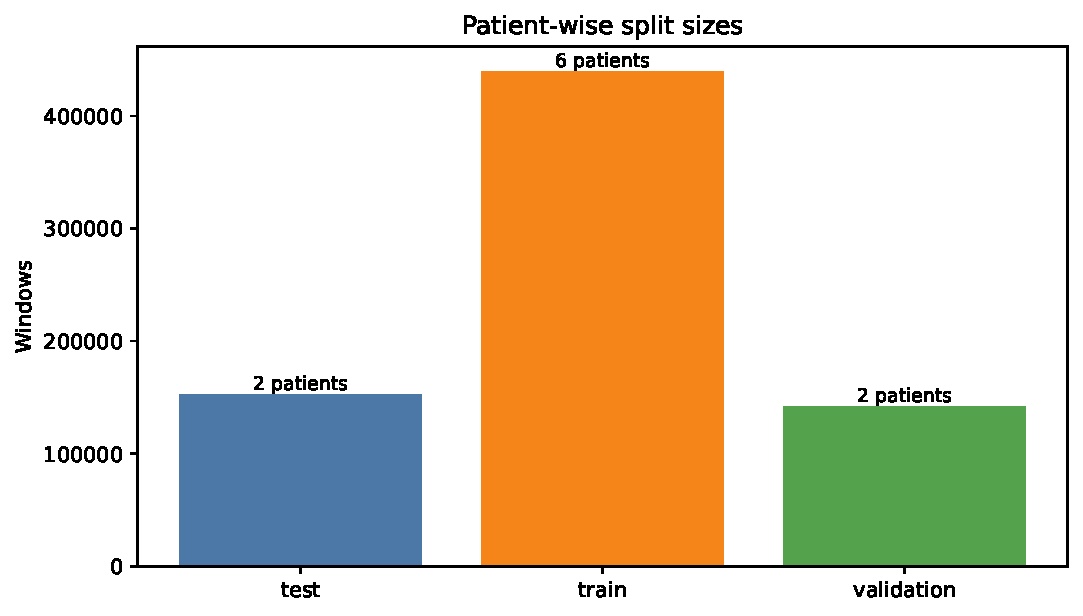
\includegraphics[width=\columnwidth]{patient_split_diagram.pdf}
\caption{Patient-wise train, validation, and test split sizes. The partitions contain disjoint patients.}
\label{fig:patientsplit}
\end{figure}

\begin{figure}[!t]
\centering
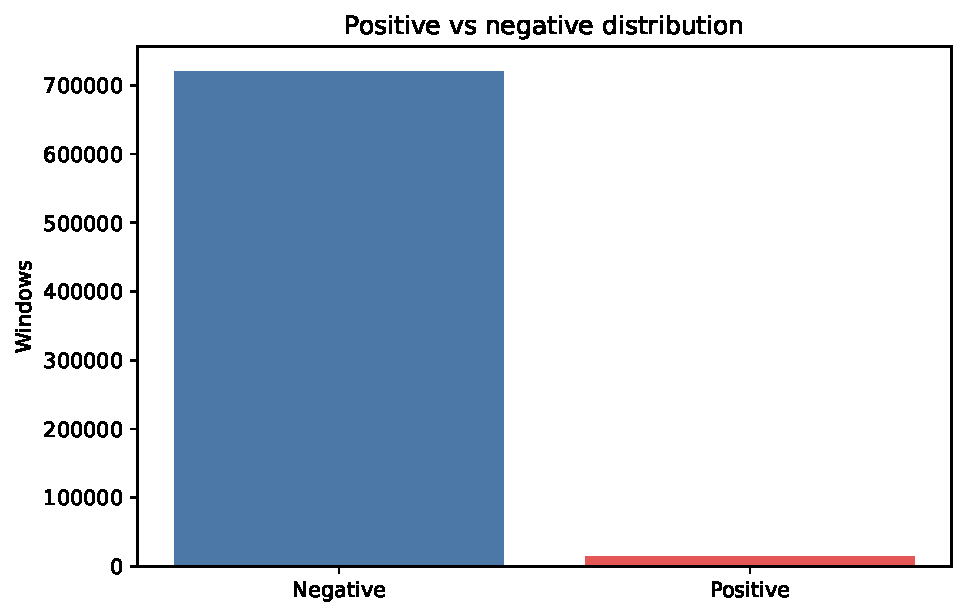
\includegraphics[width=\columnwidth]{positive_negative_distribution.pdf}
\caption{Overall positive and negative window distribution under the 10 min preictal definition. The positive prevalence is 1.9250\%.}
\label{fig:classdist}
\end{figure}

\section{Preprocessing}
Each EDF was processed independently and stored as per-EDF shards. EDF files were checked for the 18 required common EEG channels; files missing required channels were skipped. Signals were filtered using a 0.5--40 Hz bandpass filter and a 50 Hz notch filter, segmented into 4 s windows with 2 s stride, and normalized independently per window and channel using z-score normalization. The 50 Hz notch is reported as part of the frozen completed pipeline rather than as a tuned methodological claim; because CHB-MIT is a U.S. dataset where 60 Hz line noise may be relevant, this choice is treated as a limitation.

\section{Label Generation and Audit}
The primary binary label rule marks a window positive if it lies within 10 min before seizure onset. Seizure windows and the 60 s postictal exclusion interval are excluded from interictal negatives.

Table~\ref{tab:labelaudit} reports the label-audit findings. The audit found no evidence of mechanical contamination under the implemented checks. The main concern is therefore scientific label quality, not an observed coding mismatch. Early and late preictal windows receive the same label, so the positive class may be heterogeneous even when the implementation is internally consistent. Figure~\ref{fig:distance} shows the positive-window distance-to-seizure distribution.

\begin{table}[t]
\centering
\caption{Label-audit findings. Counts are from the frozen audit artifacts.}
\label{tab:labelaudit}
\begin{tabular}{lr}
\toprule
Audit finding & Value \\
\midrule
Positive windows outside implemented preictal & 0 \\
Positive windows overlapping seizure & 0 \\
Negative windows overlapping implemented preictal & 0 \\
Positive windows more than 5 min before onset & 6,685 \\
Fraction of positives more than 5 min before onset & 47.26\% \\
Median shared-overlap segment correlation & 0.9895 \\
\bottomrule
\end{tabular}
\end{table}

\begin{figure}[!t]
\centering
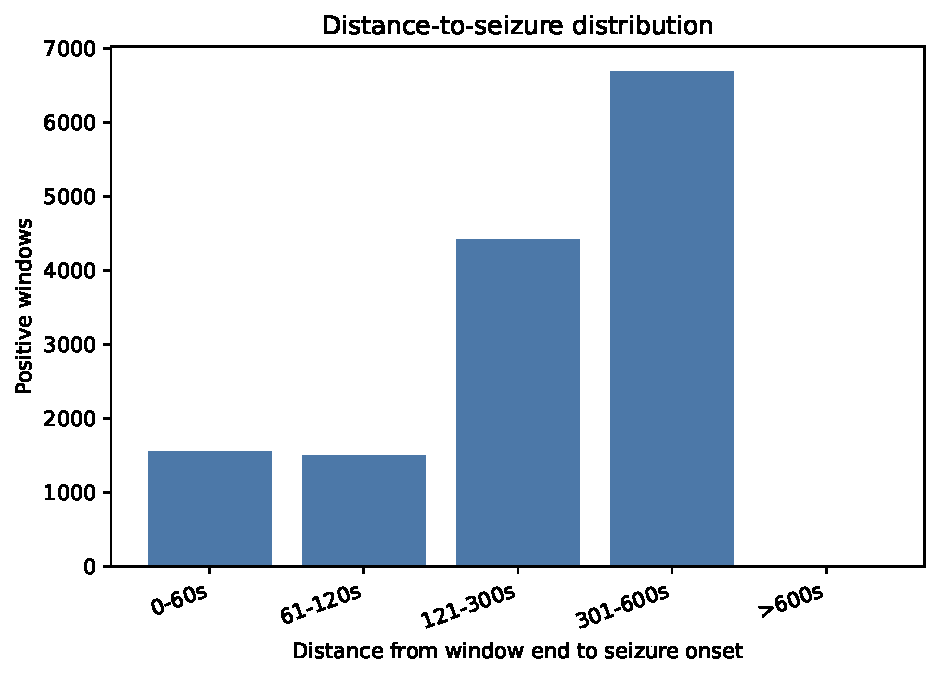
\includegraphics[width=\columnwidth]{distance_to_seizure_histogram.pdf}
\caption{Distance from positive-window end to seizure onset. A total of 47.26\% of positive windows occur more than 5 min before onset.}
\label{fig:distance}
\end{figure}

\section{Models and Training}
We evaluated EEGNet \cite{lawhern2018eegnet}, an attention-based EEG model, and a hybrid EEGNet--Transformer. EEGNet has 26,770 parameters, Attention has 13,730, and Hybrid has 295,906. The Hybrid run was time-limited and is reported as incomplete.

Training used seed 42, batch size 128, AdamW with learning rate 0.0003 and weight decay 0.0001 \cite{loshchilov2019decoupled}, ReduceLROnPlateau scheduling, automatic mixed precision on Compute Unified Device Architecture (CUDA), gradient clipping, early stopping, and checkpointing. The imbalance study evaluated weighted cross entropy, focal loss, weighted random sampling, weighted cross entropy with threshold optimization, and focal loss with threshold optimization using EEGNet. Weighted cross entropy with threshold optimization was selected by validation PR-AUC with validation F1 as the tie-breaker.

\section{Evaluation Metrics}
The primary ranking metric is PR-AUC because positives are rare. Area under the receiver operating characteristic curve (ROC-AUC), accuracy, precision, recall, F1, balanced accuracy, Matthews correlation coefficient (MCC), Cohen's kappa, sensitivity, and specificity are also reported. This study reports window-level metrics only. It does not estimate seizure-level sensitivity, false alarms per hour, time in warning, or seizure prediction horizon/seizure occurrence period metrics, which limits clinical interpretation.

\section{Results}
\subsection{Imbalance Study}
Weighted cross entropy with threshold optimization achieved validation PR-AUC 0.0239 and validation F1 0.0366 and was selected as the frozen strategy. Focal-loss variants changed threshold-dependent F1 but did not improve validation PR-AUC over the selected strategy. The weighted random sampler run was incomplete and is not used as a completed final strategy. Thus, imbalance handling changed operating points but did not produce strong ranking performance.

\subsection{Final Model Comparison}
Table~\ref{tab:modelresults} reports the final model comparison. Figure~\ref{fig:modelcomp} visualizes validation PR-AUC and F1, while Figures~\ref{fig:prcurve} and \ref{fig:confusion} provide the final EEGNet precision-recall curve and threshold-dependent confusion matrix.

\begin{table}[!t]
\centering
\caption{Final model comparison. Hybrid is included for transparency but was incomplete.}
\label{tab:modelresults}
\footnotesize
\setlength{\tabcolsep}{2.8pt}
\begin{tabular}{llcccc}
\toprule
Model & Status & Val PR & Val F1 & Test PR & Test F1 \\
\midrule
EEGNet & Completed & 0.0239 & 0.0366 & 0.0179 & 0.0258 \\
Attention & Completed & 0.0258 & 0.0000 & 0.0163 & 0.0000 \\
Hybrid & Incomplete & 0.0238 & 0.0461 & 0.0181 & 0.0354 \\
\bottomrule
\end{tabular}
\end{table}

\begin{figure}[!t]
\centering
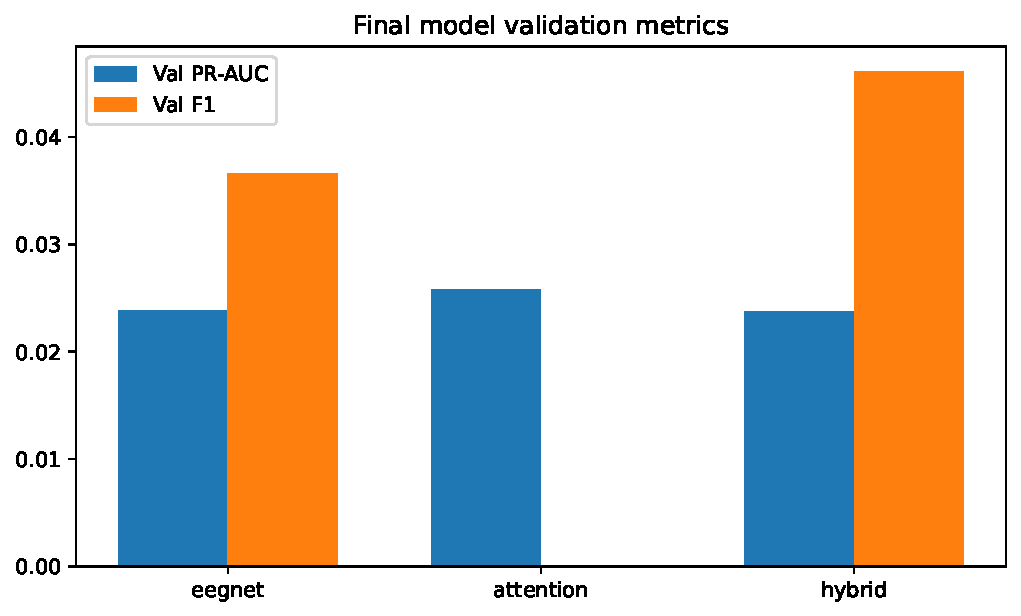
\includegraphics[width=\columnwidth]{model_comparison_chart.pdf}
\caption{Validation PR-AUC and F1 for final model runs. Hybrid is shown for transparency but was incomplete.}
\label{fig:modelcomp}
\end{figure}

\begin{figure}[!t]
\centering
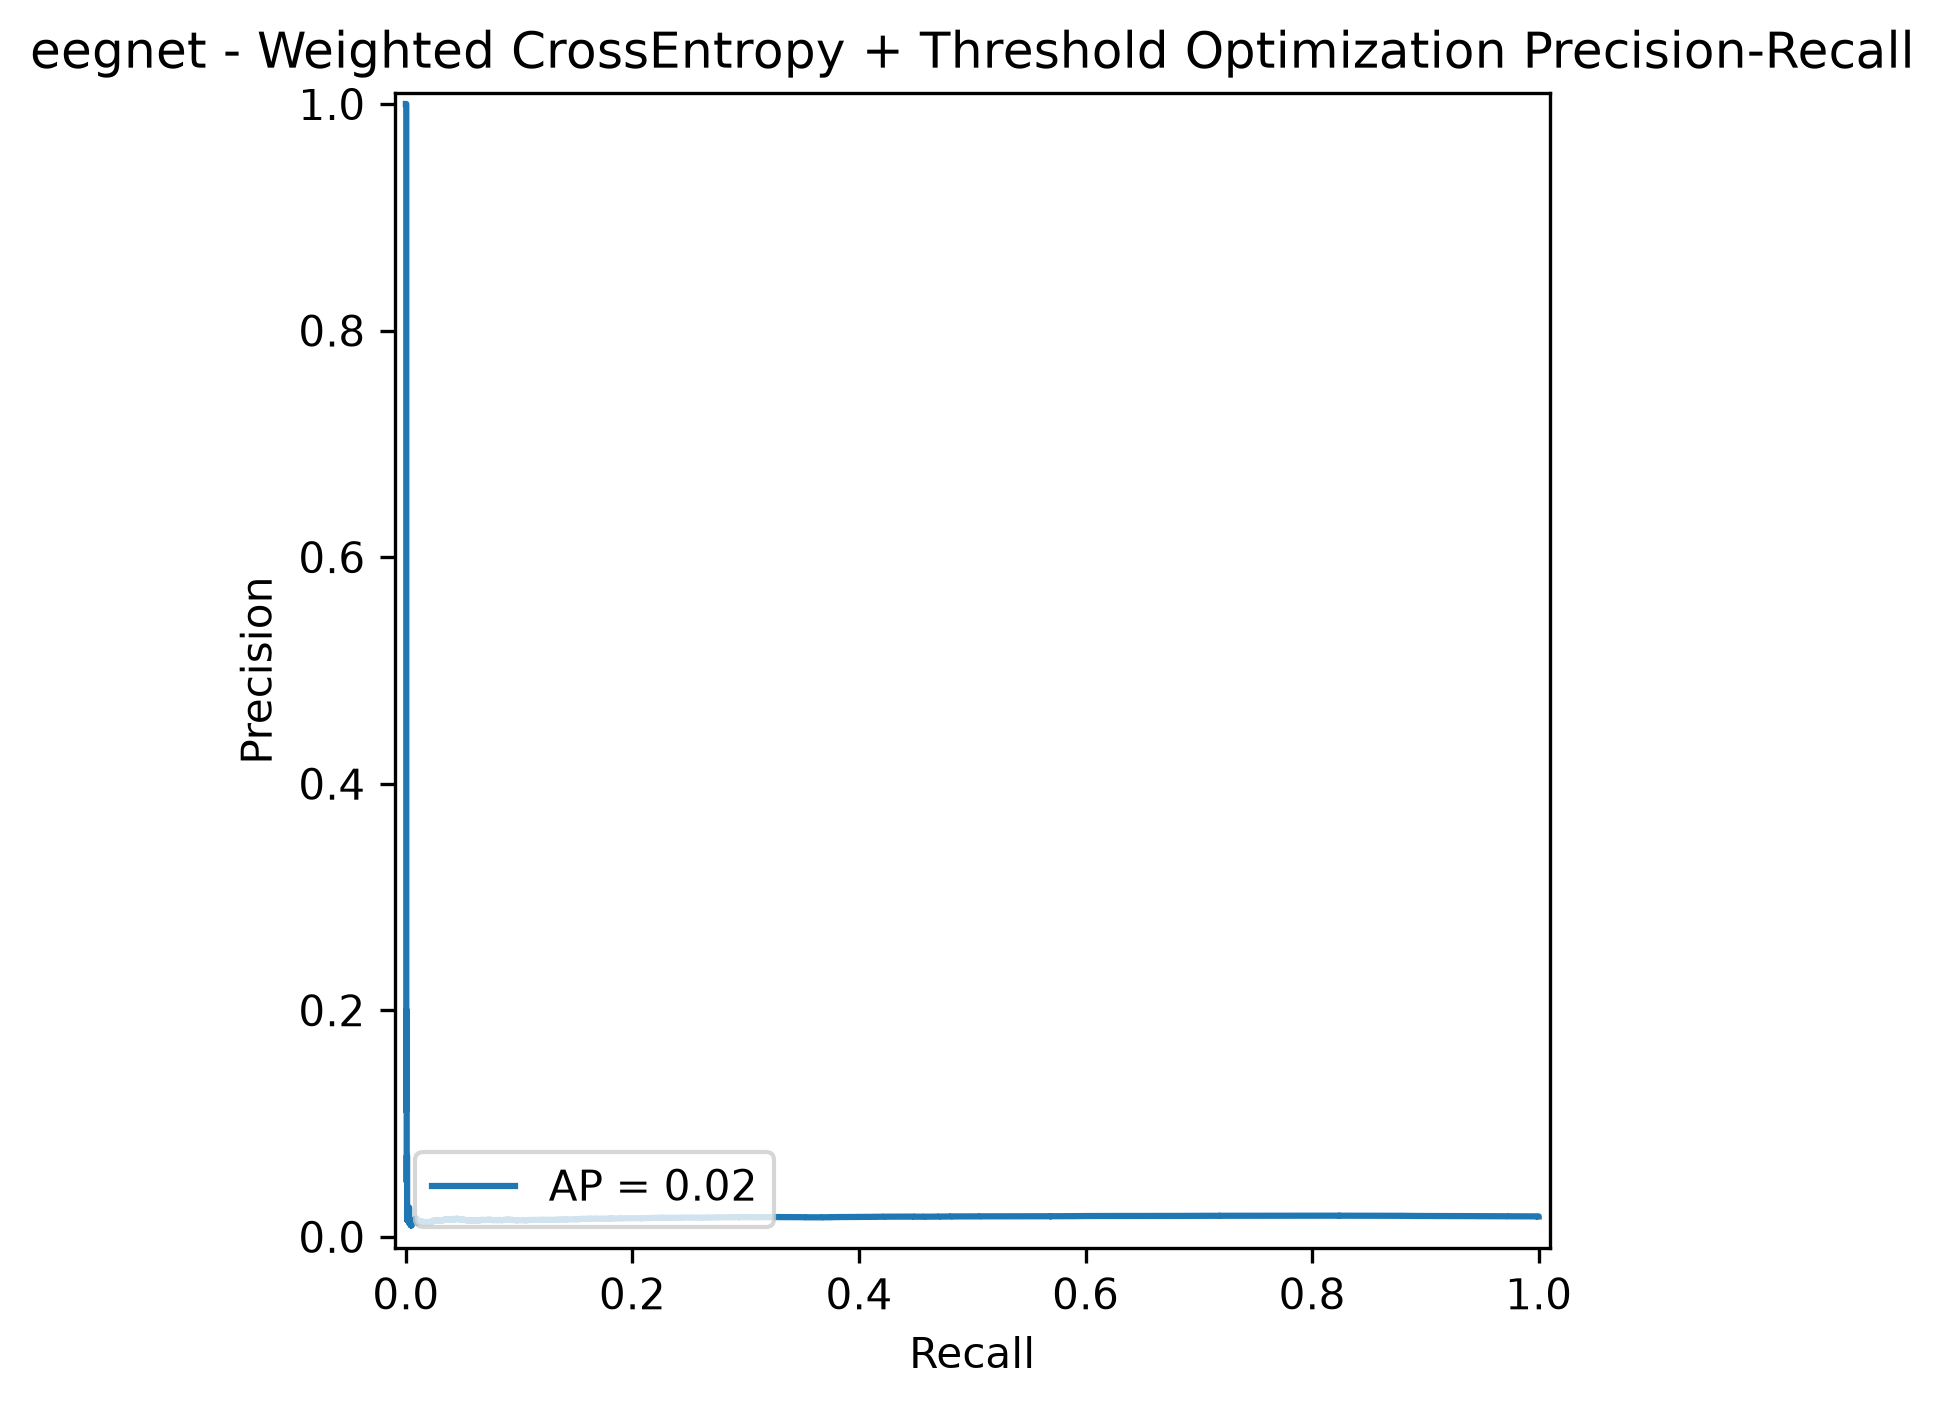
\includegraphics[width=\columnwidth]{pr_curve_eegnet.png}
\caption{Window-level precision-recall curve for the final EEGNet evaluation. PR-AUC is the primary ranking metric.}
\label{fig:prcurve}
\end{figure}

\begin{figure}[!t]
\centering
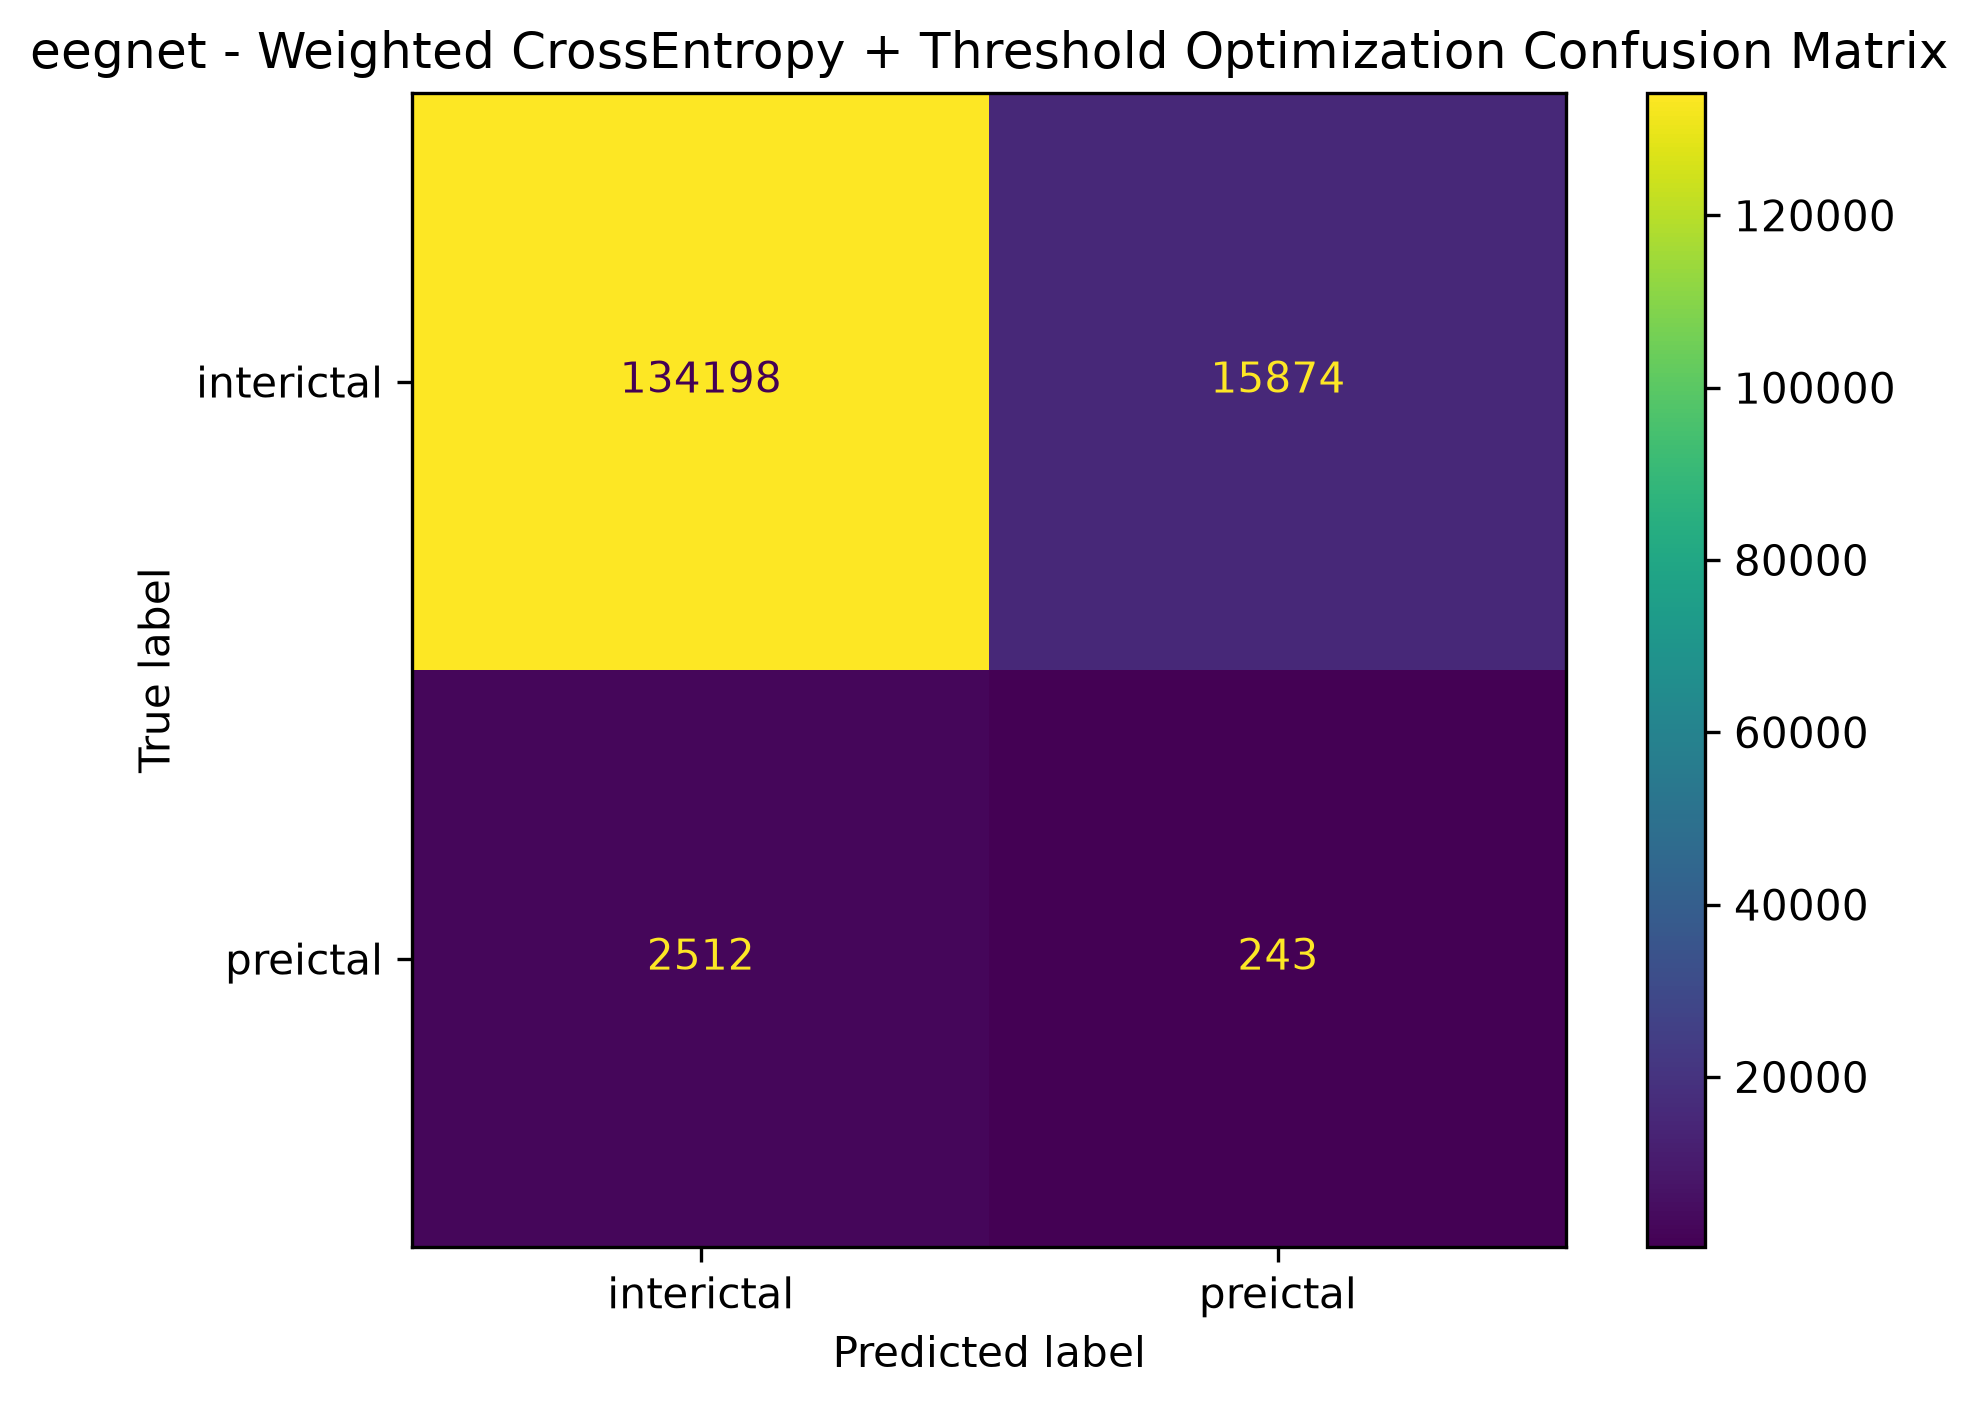
\includegraphics[width=\columnwidth]{confusion_matrix_eegnet.png}
\caption{Threshold-dependent test-set confusion matrix for the selected EEGNet operating point.}
\label{fig:confusion}
\end{figure}

None of the evaluated architectures produced validation PR-AUC substantially above the 1.9250\% positive prevalence. The Attention model's higher validation PR-AUC did not translate into nonzero F1 under the selected operating point. The available evidence does not support increased model capacity as sufficient to solve the task under this setup.

\subsection{Preictal Horizon Ablation}
Table~\ref{tab:horizon} reports the EEGNet preictal horizon ablation. Figures~\ref{fig:horizonpr} and \ref{fig:horizonf1} summarize validation PR-AUC and F1 across horizons.

\begin{table}[t]
\centering
\caption{EEGNet preictal horizon ablation. Shorter horizons reduce positives but did not improve both validation PR-AUC and validation F1.}
\label{tab:horizon}
\begin{tabular}{rrrrr}
\toprule
Horizon (min) & Positives & Prevalence & Val PR-AUC & Val F1 \\
\midrule
10.0 & 14,145 & 1.9250\% & 0.0239 & 0.0366 \\
7.5 & 10,845 & 1.4759\% & 0.0211 & 0.0271 \\
5.0 & 7,362 & 1.0019\% & 0.0140 & 0.0169 \\
3.0 & 4,422 & 0.6018\% & 0.0072 & 0.0076 \\
\bottomrule
\end{tabular}
\end{table}

\begin{figure}[!t]
\centering
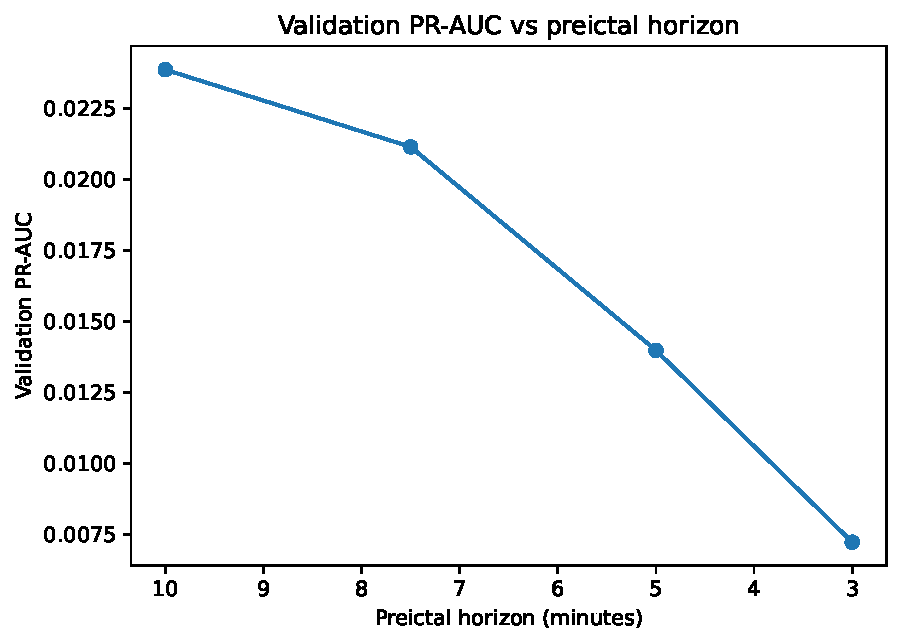
\includegraphics[width=\columnwidth]{preictal_horizon_pr_auc.pdf}
\caption{Validation PR-AUC for 10, 7.5, 5, and 3 min horizons. Shorter global horizons did not improve PR-AUC over the 10 min baseline.}
\label{fig:horizonpr}
\end{figure}

\begin{figure}[!t]
\centering
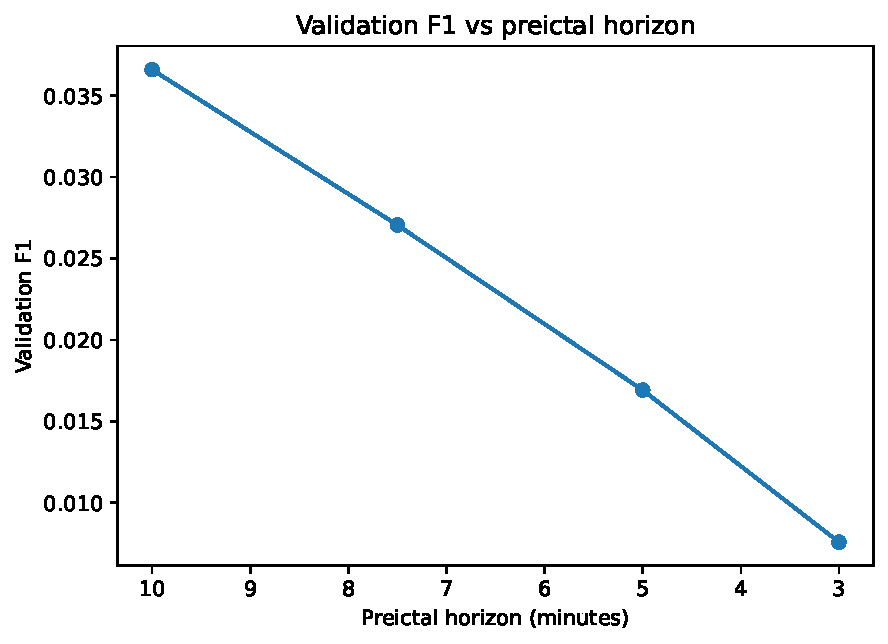
\includegraphics[width=\columnwidth]{preictal_horizon_f1.pdf}
\caption{Validation F1 for 10, 7.5, 5, and 3 min horizons. Shorter global horizons did not improve F1 over the 10 min baseline.}
\label{fig:horizonf1}
\end{figure}

Simple global horizon shortening was not sufficient to improve discrimination. This does not prove that preictal label design is irrelevant; it only shows that the tested global horizons did not improve the measured validation metrics.

\FloatBarrier

\section{Discussion}
The central finding is a bounded negative result: under a patient-wise split and the completed preprocessing protocol, standard imbalance handling, threshold optimization, and the evaluated neural architectures did not produce reliable window-level seizure prediction.

The preprocessing and data audits matter because EEG seizure prediction pipelines are vulnerable to silent failure modes. If seizure windows, postictal windows, duplicate windows, or patient identities leak across splits, performance can appear artificially strong. The audit trail reduces this risk and makes the negative result more interpretable.

The label audit matters because poor performance across multiple model and loss configurations suggested that the bottleneck might be in the target definition. The audit found no evidence of mechanical label contamination, but it did show that nearly half of positive windows were more than five minutes before onset. This supports caution about broad fixed preictal labels, although the subsequent horizon ablation did not show that shortening the horizon alone improves performance.

The negative findings are scientifically useful because they constrain future work. They suggest that simply adding capacity, reweighting losses, or shortening a global horizon may be insufficient for patient-wise CHB-MIT seizure prediction from isolated 4 s raw EEG windows.

\section{Limitations}
This study has important limitations: only 10 CHB-MIT patients and 50 seizures were included; evaluation uses a single patient-wise split rather than leave-one-patient-out or repeated patient-wise splits; no confidence intervals, bootstrap intervals, or repeated-seed variance estimates are available; metrics are window-level rather than seizure-level or alarm-level; overlapping windows introduce redundancy; the models classify isolated windows rather than longer temporal sequences; the Hybrid run was incomplete; the 50 Hz notch filter may not be optimal for CHB-MIT; and no classical feature-based baselines were evaluated.

\section{Future Work}
Future work should evaluate leave-one-patient-out validation, repeated seeds, confidence intervals, seizure-level sensitivity, false alarms per hour, time-in-warning, explicit seizure prediction horizon and seizure occurrence period definitions, patient-specific preictal horizons, stricter interictal sampling, longer temporal context, classical feature-based baselines, and line-noise filtering choices.

\section{Conclusion}
This study provides a repository-backed patient-wise CHB-MIT seizure prediction experiment with leakage, label, imbalance, and horizon audits. The measured results do not support claims of strong predictive performance: validation PR-AUC remained close to positive prevalence, and no tested shorter preictal horizon improved both PR-AUC and F1 over the 10 min baseline. The main contribution is an honest, reproducible negative finding that highlights the importance of label definition, patient-wise evaluation, and clinically meaningful metrics in seizure prediction research.

\FloatBarrier
\bibliographystyle{IEEEtran}
\bibliography{../references/references}
\end{document}
